\chapter{System Design and Implementation}

\section{Global System Design}
In this section, we will explain how we designed the application and why we made several decisions.
We do this with different diagrams.
We have made for example a class diagram, a database diagram, sequence diagrams and state diagrams.

\subsection{Database}
In Figure~\ref{database_diagram}, you see our database diagram.
We will explain the structure of the database shortly.

\begin{figure}[h]
    \centering
    \captionsetup{justification=centering}
    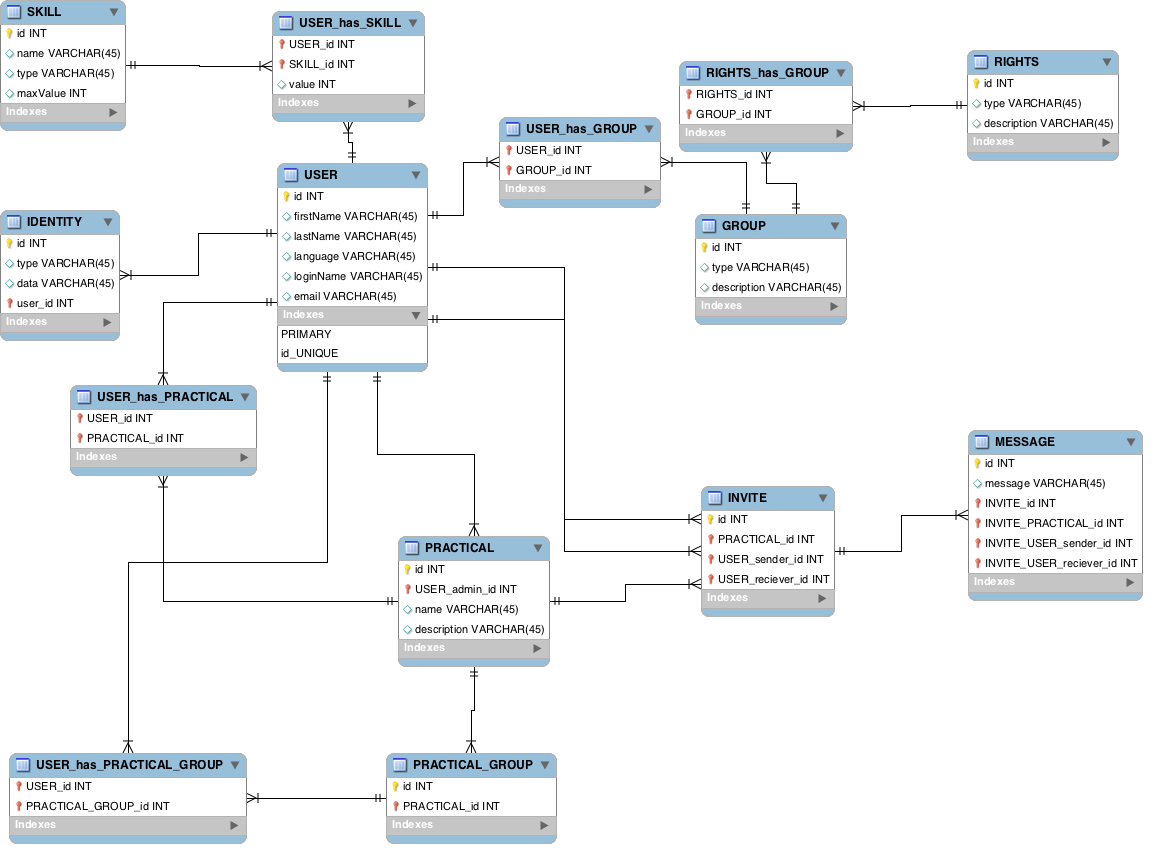
\includegraphics[width=\textwidth, frame]{images/database_diagram}
    \caption{The database diagram}
    \label{database_diagram}
\end{figure}

\noindent In the center of the diagram, you see the user.
The user has a many to many relation with a group.
There are four different groups.
There is a group for students, for teachers, for administrators and one for guests.
It is obvious that a group can contain multiple users, but a user can also have multiple groups.
Users can be a teacher, as well as an administrator.

Every group has different rights.
The same right can also be assigned to multiple groups.
That is why we also have a many to many relation between a group and a right.
\\\\
A user must also be able to log in.
To accomplish this, the user must have an identity.
An identity can only belong to one user.
If this should not be the case, the system would not be save because other users have access to a user's rights.
\\\\
A user can be part of multiple practical groups and a practical group consist of multiple users.
Therefore, user and practical group have also a many to many relation.
This is the same for user and practical.

A practical group belongs to only one practical.
A practical group does not belong to multiple practicals.
\\\\
An invite has two many to one relations with a user.
An invite has a sender as well as an receiver.
There can only be one sender and one receiver for an invite.

Every invite belongs to only one practical.
These therefore have also a many to one relation.
\\\\
The last relation is between an invite and a message.
These messages are for communication between the sender and the receiver of the invite.
An invite can have multiple messages.
Every message belongs to only one invite.

\section{Model View Controller}
As mentioned earlier, we are using the Play Framework. 
This frameworks follows the Model View Controller (MVC) architectural pattern applied to the Web architecture\cite{playframework_mvc}.
This pattern splits the application into separate layers: the Presentation layer and the Model layer. 
The Presentation layer is further split into a View and a Controller layer.

\subsection{Controller}
The \textbf{Controller} responds to events (typically user actions) and processes them, and may also invoke changes on the model.
In a Web application, events are typically HTTP requests: a Controller listens for HTTP requests, extracts relevant data from the 'event', such as query string parameters, request headers... 
And applies changes on the underlying model objects.
\\\\
In Play, a Controller is a Java class where each public, static, method is an \textbf{action}.
An action is a Java entry point invoked when a HTTP Request is received.
The Java code from the Controller class is not really object oriented: it is mainly procedural code.
The action method extracts relevant data from the HTTP request, reads or updates the model objects, and sends back a result which is wrapped into an HTTP Response.

\subsection{Model}
The \textbf{Model} is the domain-specific representation of the information on which the application operates.
Domain logic adds 'meaning' to raw data (e.g., calculating if today is the user's birthday, or the totals, taxes, and shipping charges for a shopping cart).
 Most applications use a persistent storage mechanism such as a database to store data.
MVC does not specifically mention the data access layer because it is understood to be underneath, or encapsulated by, the Model.
\\\\
In Play, the domain model object layer is a set a Java classes using all the object oriented features available from the Java language. 
It contains data structures and operations on which the application operates. 
Whenever model objects need to be saved into a persistent storage, they may contain some glue artefacts like JPA annotations or SQL statements.

\subsection{View}
The \textbf{View} renders the model into a form suitable for interactions, typically a user interface.
Multiple views can exist for a single model, for different purposes.
In a Web application the view is usually rendered in a 'Web format' like HTML, XML or JSON.
However there are some cases where the view can be expressed in a binary form, e.g. dynamically rendered chart diagrams.
\\\\
In Play, most of the application views are generated using an efficient template system provided by play. 
The Controller gets some interesting data from the model layer, and then applies a template to decorate these objects. 
This packages contains HTML, XML, JSON and other template files with special directives used to dynamically generate the model representation.
\\
\begin{figure}[h]
  \centering
    \captionsetup{justification=centering}
    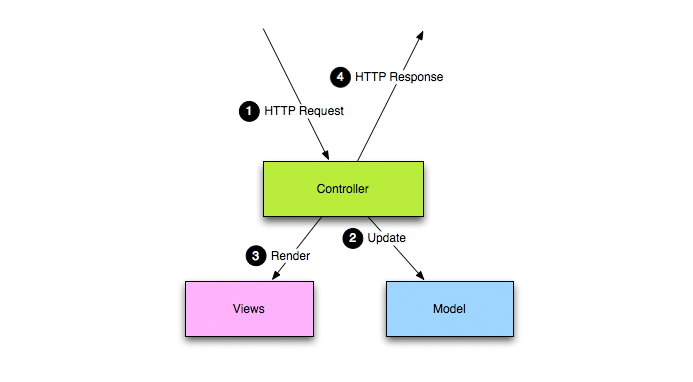
\includegraphics[width=\textwidth]{play_mvc}
    \caption{Play Framework MVC structure}
  \label{play_mvc_image}
\end{figure}


\section{Implementation}
In this section we will describe the software implementation of APMatch.
We will start of with some global implementation description of our APMatch system and then we will continue with some more advanced topics.

We chose to explain some more about both the invites and the matching algorithm.
For the invites we explain what are difficulties were and which situations were hard to implement, while for the matching algorithm we will explain some more how it works and why we chose it.

\subsection{Global}

\subsection{Invites}

\subsection{Matching algorithm}
For our matching algorithm we used our custom designed algorithm.
This algorithm uses the skills defined by the user and the teacher to find the best matching with the preferences of the teacher.
We will first give a description of the algorithm followed by a formal description.
After that we will give a description about the complexity and will conclude this section with why we chose this implementation.

Before we start explaining the algorithm we will first describe how to calculate the distance for a certain practical group.
Calculating the distance of a practical group is done by going through the skills defined by the practical teacher.
We will then calculate the average of the values of the skills of all the users in the practical group and the users' practical group combined.
Then all the average's are multiplied with each other and then you take root of the amount of skills in the practical.
This resulting number will defined as the distance.

The matching algorithm starts with a practical and user.
It will start with going through the different practical groups in the practical.
To simplify the algorithm it is chosen to make sure every user is in a practical group.
This means that when an user doesn't have any practical partners he is still in a practical group with only himself in it.
While going trough the different practical groups it will calculate the distance as described in the previous paragraph.
After calculating the distance with every other practical group and saving this in a map, this result is sorted by descending distance.
Then we start recommending practical groups to the user starting by the top of the list.
The formal definition of this algorithm is visible in Algorithm \ref{recommend}.

\begin{algorithm}
\begin{algorithmic}
\Function{Recommend}{$practical$, $user$}
	\State $resultList\gets$ Empty map of PracticalGroup and distance
	\ForAll{$practicalGroups$ in the $practical$}
		\State $distance\gets 0$
		\ForAll{$skills$ in the $practical$}
			\State $average\gets 0$
			\ForAll{$users$ in the $practical$}
				\State $average\gets average + SkillValue(user, skill)$
			\EndFor
			\ForAll{$users$ in the $user$ practical group}
				\State $average\gets average + SkillValue(user, skill)$
			\EndFor
			\State $average\gets average / (amount\_of\_users)$\Comment{The amount of users in the practical}
			\State $distance\gets distance * (average - SkillValue(Practical, Skill))$
		\EndFor
		\State $distance\gets distance ^ {(1 / amount\_of\_skills)}$\Comment{The amount of skills in the practical}
		\State $resultList\gets resultList + (practicalGroup, distance)$
	\EndFor
	\State Sort the $resultList$ by descending $distance$
	\State \textbf{return} $resultList$
\EndFunction
\caption{The recommendation algorithm}\label{recommend}
\end{algorithmic}
\end{algorithm}

To Analyse the complexity we need the following measurements.
We define $n$ as the amount of practical groups in a practical.
We define $m$ as the amount of skills defined in a practical.
We define $j$ as the amount of users in a certain practical group plus the amount of users in your own practical group.
Since in the first loop we go trough the practical groups to calculate the distance we start with a time complexity of $O(n)$.
Inside this loop we go trough each of the skills defined in the practical to calculate the average which will give us $O(n*m)$.
In order to calculate this average we need to go rough all the users in our practical group and the practical group examined.
This will lead to a time complexity of $O(n*m*j)$.
As one of the last steps we still need to sort the list of the practical groups which will be done in a time complexity of $O(n*log(n))$.
All this combined will lead into a total time complexity of $O(nmj+n*log(n))$ which for small $m$ and $j$ will lead to a total time complexity of $O(n*log(n))$.

We chose this implementation, because it is very easy to understand and very adjustable implementation of the algorithm.
There are several ways to optimise the algorithm by using precomputing.
This can be done for example during the defining of the skills by the user and will save execution time when viewing recommended solutions.
Next to that we have shown in the previous paragraph that with both a small amount of skills defined by a practical and with a small amount of users in practical groups, this algorithm will run in $O(n*log(n))$.
Since this will be the case, because both sizes are limited this will be fast enough to run while recommending without precomputing.
All these cases prove that the algorithm is good enough for recommendation system.



